\chapter{Multi-vessel System State Description}
\label{chap:stateDescription}
This chapter builds on existing vessel state descriptions to formulate a multi-vessel state description. Furthermore, a novel approach to predict multi-vessel platform dynamics from individual models is proposed to  answer the research subquestion:

\begin{itemize}
	\item How can the dynamics of the multi-vessel system be represented?
\end{itemize}
The described multi-vessel state description as described in Sec. \ref{sec:notations} aims to enable consistent system notation of scenarios pertaining more than a single vessel, as mult-vessel frameworks have more objects that can be referred to. The concept and definition of a platform-coordinate system is also introduced.

For collaborative motion control of modular objects an approximate dynamical model is often desired. As model parameter estimation experiments are often infeasible for every configuration of a combined structure, a prediction of dynamical behavior is proposed using the often known dynamics of modules in Sec. \ref{platformModel}

\section{System State Notations} 
\label{sec:notations}
A sensible notation of a system aids implementation and consistent discussion of motion control systems. Vessel automation is a topic where robotic and maritime science overlap. System description of vessel systems from a control perspective is described in \citet{fossen2011handbook}, which are used as a foundation of the multi-vessel state description

\subsection{Single vessel state description}
For control purposes, ships are generally considered rigid bodies. A rigid body has 6 degrees of freedom (DOF) in which can all be evaluated or simplified to a reduced set of motions such as 3-DOF planar motion. For ships, this is commonly expressed according to the notation of \citet{sname1950nomenclature} with respect to various coordinate systems. Components of orientation, velocities and forces are shown in table \ref{tableSname}.

\begin{table}[h!]
	\centering
	\begin{tabular}{|l|l|l|l|l|}
		\hline
		DOF & & \begin{tabular}[c]{@{}l@{}}Positions and \\ Euler Angles\end{tabular} & \begin{tabular}[c]{@{}l@{}}Linear and \\ angular Velocities\end{tabular}   & \begin{tabular}[c]{@{}l@{}}Forces and \\ Moments\end{tabular}  \\ \hline
		1&	Surge      & x                    & u          & X                  \\ \hline
		2&	Sway       & y                    & v          & Y                  \\ \hline
		3&	Heave      & z                    & w          & Z                  \\ \hline
		4&	Roll       & $\phi $                 & p          & K                  \\ \hline
		5&	Pitch      & $\theta  $              & q          & M                  \\ \hline
		6&	Yaw        & $\psi  $                & r          & N                \\ \hline
		
	\end{tabular}
	\caption{SNAME notation for marine vessels}
	\label{tableSname}
\end{table}

A North-East-Down coordinate system will be used as reference to a global coordinate system as $\{n\}$, while a body fixed coordinate system is referred to with $\{b\}$. This body fixed frame defines the motion of the vessel, such that every position or speed of a vessel is defined in the motion of the body frame. Figure \ref{figsname} shows vessel motions expressed on the body fixed frame. Motion of surface vessels is commonly simplified to 3 degrees of freedom in the surface plane, as is shown in figure \ref{fig:delfiaBodyFrame1}. This assumes effects of heave, roll and pitch can be neglected. This simplification of planar motion is adopted for the developed control system in this paper as described in Chap. \ref{chap:sysDevelopent}. 

\begin{figure}[h!]
	\centering
	\makebox[\textwidth][c]{
		\begin{minipage}{0.45\textwidth}
	\centering
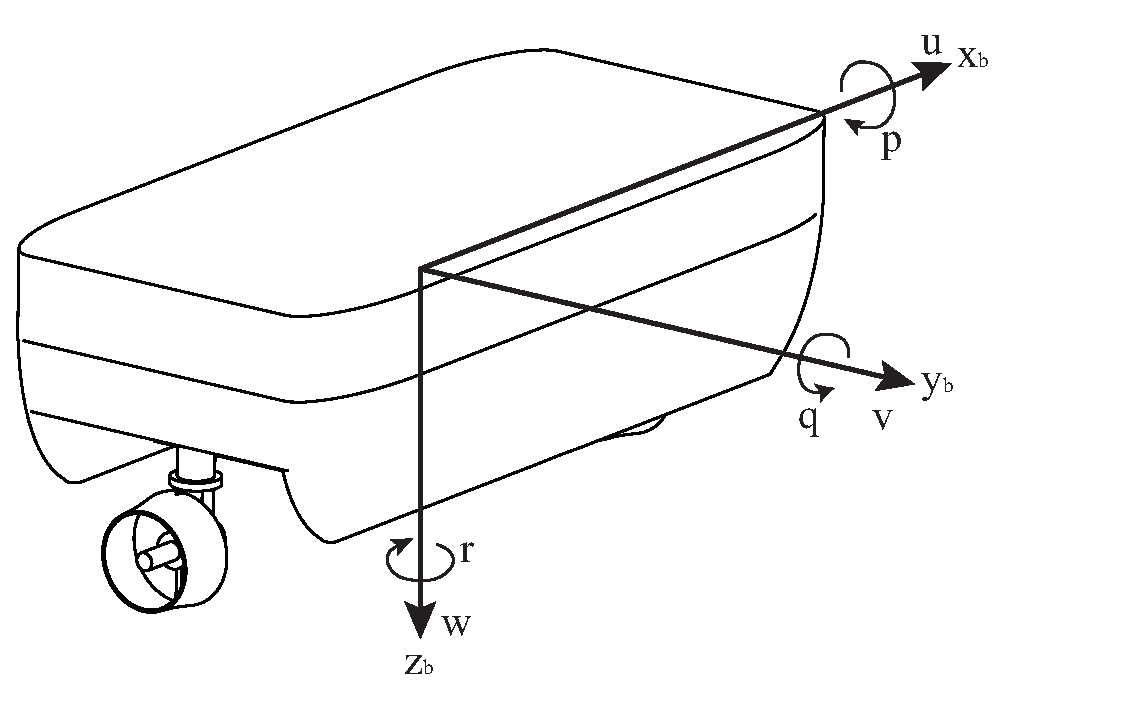
\includegraphics[width=1.0\textwidth]{DelfiaSname.eps}
\caption{Six degrees of motion depicted of a Delfia vessel expressed with respect to the body-fixed coordinate system $\{b\}$ in convention with \citet{sname1950nomenclature}}
\label{figsname}
		\end{minipage}\hfill
		\begin{minipage}{0.45\textwidth}
	\centering
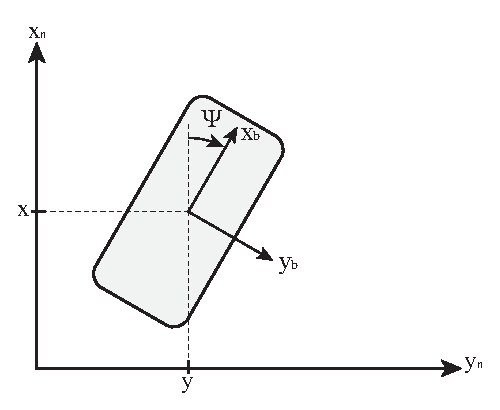
\includegraphics[width=1.0\textwidth]{delfia_bodyframe1.eps}
\caption{Three degrees of freedom depicted as only motion in the surface plane is considered}
\label{fig:delfiaBodyFrame1}
		\end{minipage}
	}
\end{figure}

Position, orientation, velocities, forces and moments are further noted as:
\begin{table}[H]
\centering
\begin{tabular}{lll}
		$\textbf{p}^{i}_{j} $ 			& = &  	Position of point $j$ expressed in coordinate system $\{i\}$ \\[5pt]
		$\Theta_{ij}$ 					& = & 	Euler angles between coordinate systems $\{i\}$ and $\{j\}$ \\[5pt]
		$ \textbf{v}^{k}_{i/j}$   		& = & 	Linear velocity of point i with respect to j expressed in coordinate system $\{k\}$ \\[5pt]
		$ \omega^{k}_{i/j}$   			& = &	Angular velocity of object i with respect to j expressed in coordinate system $\{k\}$  \\[5pt]
		$\boldmath{f}^{i}_{j} $ 	   	& = &	Force with line of action through point $j$ expressed in coordinate system $\{i\}$ \\[5pt]
		$\boldmath{m}^{i}_{j} $   		& = & 	Moment about point $j$ expressed in coordinate system $\{i\}$
\end{tabular}
\end{table}

As a result of the reduction from 6 to 3 degrees of freedom, vectorial expressions of our system become:
\begin{table}[H]
	\centering
	\begin{tabular}{llllllll}
		NED position & $\textbf{p}^{n}_{b} $ & = & $  \begin{bmatrix} x^{n}_{b} \\[5pt] y^{n}_{b} \end{bmatrix}$ & 
		Attitude (Euler angles) & $\Theta_{nb} $ & = & $ \begin{bmatrix} \Psi^n_b \end{bmatrix}$   \\[20pt] %\begin{bmatrix} N \\ E \end{bmatrix} =
		\begin{tabular}[c]{@{}l@{}}Body-fixed \\ linear velocity \end{tabular} & $ \textbf{v}^{b}_{b/n} $ & = & $ \begin{bmatrix} u \\ v \end{bmatrix} $ & 
		\begin{tabular}[c]{@{}l@{}}Body-fixed \\ angular velocity \end{tabular} & $ \omega^{b}_{b/n} $ & = & $ \begin{bmatrix} r \end{bmatrix} $ \\[20pt]
		\begin{tabular}[c]{@{}l@{}}Body-fixed \\ force \end{tabular} & $\boldmath{f}^{b}_{b} $ & = & $ \begin{bmatrix} X \\ Y \end{bmatrix} $ & 
		\begin{tabular}[c]{@{}l@{}}Body-fixed \\ moment \end{tabular} & $\boldmath{m}^{b}_{b} $ & = & $ \begin{bmatrix} N \end{bmatrix} $ 
	\end{tabular}
\end{table}


General motion of vessels in 3 degrees of freedom are described by the following generalized positions and velocities \cite{fossen2011handbook}

\begin{equation}
	\eta = \begin{bmatrix} \textbf{p}^{n}_{b} \\[8pt]  \Theta_{nb} \end{bmatrix} = \begin{bmatrix} x^{n}_{b} \\[8pt]  y^{n}_{b} \\[8pt] \Psi^n_b \end{bmatrix}
	\label{generalizedPos1}
\end{equation}

\begin{equation}
	\nu = \begin{bmatrix} \textbf{v}^{b}_{b/n} \\[8pt]  \omega^{b}_{b/n} \end{bmatrix} = \begin{bmatrix} u\\v\\r \end{bmatrix}
	\label{generalizedVel1}
\end{equation}

\begin{equation}
	\tau = \begin{bmatrix} \boldmath{f}^{b}_{b} \\[8pt]  \boldmath{m}^{b}_{b} \end{bmatrix} = \begin{bmatrix} X \\ Y \\ N \end{bmatrix}
	\label{generalizedFor1}
\end{equation}

Where $\eta$ describes orientation, $\nu$ describes velocities and $\tau$ describes forces acting upon the system. 
To avoid clutter, when it is deemed clear to in which reference frame a position or velocity is expressed, the subscript and superscript will not always be shown. This is for instance the case for generalized positions as in equation \ref{generalizedPos1} that is most of the time with respect to $\{n\}$ such that it is just expressed in $ [x,y,\Psi]^\top$. By default, $ \nu$, $\tau$ are expressed in $\{b\}$, and $\eta$ is described in $\{n\}$.

Velocities expressed in $\{b\}$ and $\{n\}$ frame are related as:

\begin{equation}
\dot{\eta} = R(\Psi)\nu
\end{equation}

Where $R$ is the rotation matrix of $\Psi$ around the z axis. For pure motion in the 3 surface plane degrees of freedom, this becomes:

\begin{equation}
R(\Psi) = \begin{bmatrix} cos(\Psi) & -sin(\Psi) & 0  \\ sin(\Psi) & cos(\Psi) & 0 \\ 0 & 0 & 1 \end{bmatrix}
\end{equation}

Coordinate system origin and centre of mass are referred to as:

\begin{table}[H]
	\centering
	\begin{tabular}{lll}
		$\textbf{o}_{i}^{j} $ 			& = &  	Origin of coordinate system $i$ expressed in coordinate system $\{j\}$ \\[10pt]
		$\textbf{p}_{cm}^{i} $ 			& = &  	Position of the centre of mass expressed in coordinate system $\{i\}$ \\
	\end{tabular}
\end{table}


\subsection{Multivessel system notation}
As fleet systems transition from describing a single vessel to a system of many, it becomes necessary to differentiate between local frames of different vessels. We change subscripts referencing to a single vessel to a notation for $n$ vessels. For example, referencing to a single body coordinate system as $\{b\}$ changes to $\{b1\},\{b2\},\{b2\} \dots \{bn\}$ in order to indicate which body frame is referenced to. Relative orientations and velocities are considered to become more relevant as vessels have to operate in proximity or even contact to realize assembly into platforms. Figure \ref{fig:localframeShowing} illustrates how position of a vessel can be described in a local body fixed frame, which may be more relevant and intuitive for automated assembly purposes. The position of origin of body 2 expressed in $\{b1\}$ illustrated in figure \ref{fig:localframeShowing} becomes:

\begin{equation}
\textbf{o}_{b1}^{b2} = \begin{bmatrix}x_{b1}^{b2} \\[10pt] y_{b1}^{b2} \end{bmatrix}
\end{equation}

Furthermore, the notations of motion shown in equation \ref{generalizedPos1}, \ref{generalizedVel1} and \ref{generalizedFor1} by default refer to a specific frame. Pose $\eta$ is expressed globally in $\{n\}$. Velocities $\nu$ and  forces $\tau$ are expressed in the body fixed frame $\{b\}$. It can be convenient to express motions to different frames as well. Take the example of two moving vessels docking to eachother while moving. To answer the question "How close is a vessel to a docking position?" a relative expression of position is required. The convention of subscripting to refer to a coordinate system is extended to $\eta$, $\nu$ and $\tau$ as well as follows:

\begin{equation}
\eta_b^n = \begin{bmatrix} \textbf{p}^{n}_{b} \\[8pt]  \Theta_{nb} \end{bmatrix} = \begin{bmatrix} x^{n}_{b} \\[8pt]  y^{n}_{b} \\[8pt] \Psi^n_b \end{bmatrix}
\label{generalizedPos2}
\end{equation}

Where the sub- and superscript of $\eta_b^n$ refer to object $b$ expressed in $\{n\}$. This convention allows expression of relative motion between vessels by writing $\eta_{b2}^{b1}$ which indicates pose of body 2 expressed in the local frame of body 1, also illustrated in \ref{fig:localframeShowing}. Note that velocities and forces are regularly referred to as "body-fixed", but that is not necessarily the case anymore with this convention. 

\begin{figure}[h!]
	\centering
	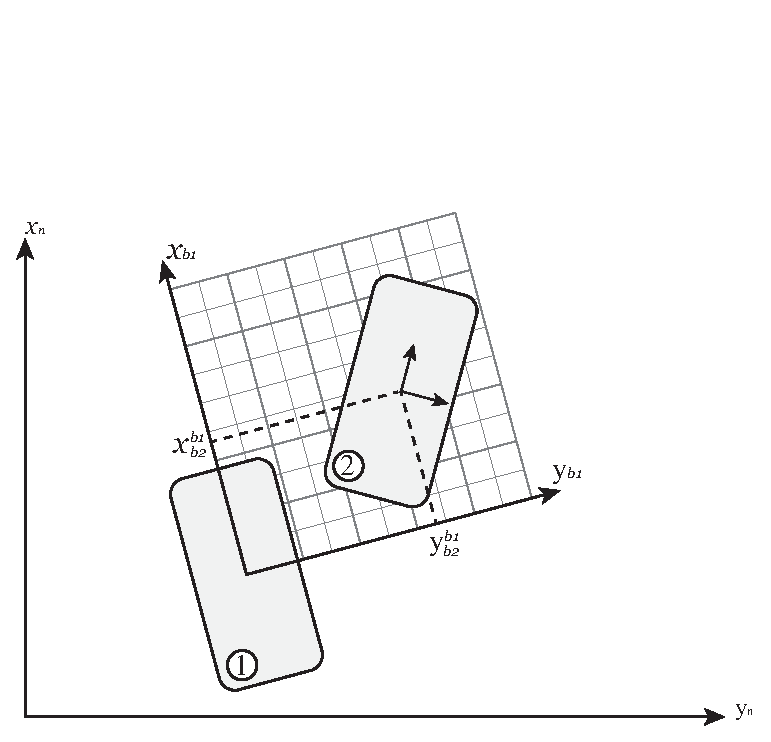
\includegraphics[width=0.6\textwidth]{localframeShowing.eps}
	\caption{Two vessels are shown from above, illustrating interpretation of expressing a module's state (of module 2) in another module's body-fixed coordinate system (of module 1).}
	\label{fig:localframeShowing}
\end{figure}
\newpage

\section{Dynamical model of a Platform}
\label{platformModel}
An approximate model for the platform dynamics is used by the platform controller in the process of generating control effort. When the platform control agent is notified that its configuration is changed, it recomputes various parameters for the dynamical model that describe the new rigid body dynamics.
The platform control agent keeps track of the following 
\begin{itemize}
	\item Connectivity of modules
	\item Configured pose connected modules
	\item Parameters that describe dynamics of individual modules
\end{itemize}

Use-cases where vessel assemblies are formed in many varying configurations can make experimental model parameterization infeasible for all reasonably forseeable configurations.  Predicting a dynamical model by combining models of modules can provide a quick, cheap and scalable solution with respect to performing parameter estimation experiments. 
The approach to estimating the dynamical model of a platform is explained in this section, but also more elaborately described and discussed in appendix \ref{appendix:CombineDynamics}

A dynamic model of the platform is formed by expressing all models of the modules in the same point and coordinate system, which are then combined. It is shown how terms from multiple module models can be grouped for convenient expression, and how the centre of mass of the combined structure can be found. 

Models of modules are expressed in platform frame origin by (1) translating the expressions to $o_{p}$ as a reference point and (2) rotating the expressions to match  coordinate system $\{p\}$. This approach works also for models of which the origonal inertial matrix is not defined in the CG, and/or for models that have directional dependent mass (e.g., hydrodynamic added mass). 

Generalized positions and velocities of the platform are described respectively as
\begin{equation}
	\eta_{p/n}^{n} = \begin{bmatrix} \textbf{p}^{n}_{p} \\[8pt]  \Theta_{np} \end{bmatrix}
\end{equation}
\begin{equation}
	\nu_{p/n}^{p} = \begin{bmatrix} \textbf{v}^{p}_{p/n} \\[8pt]  \omega^{p}_{p/n} \end{bmatrix}
\end{equation}

\begin{figure}[H]
	\centering
	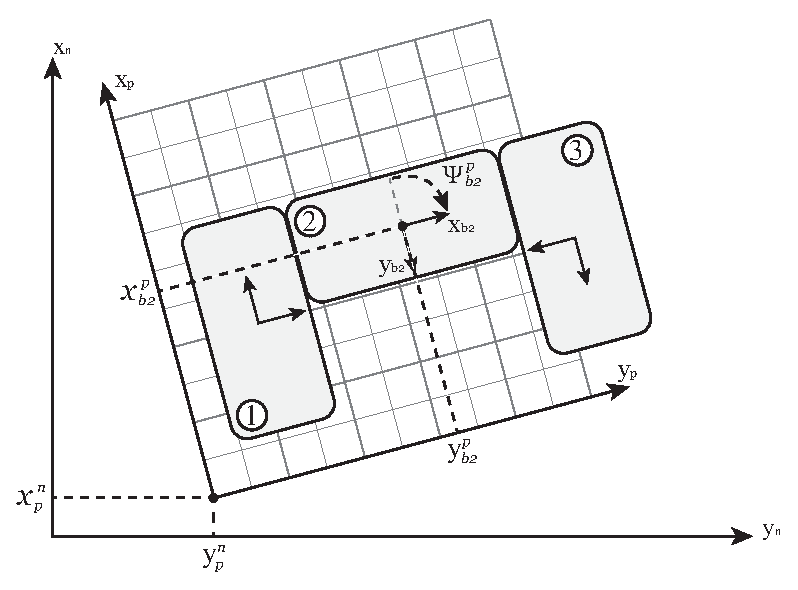
\includegraphics[width=0.7\textwidth]{ned_platform_frame}
	\caption{An assembly of three vessels in 2d. Components from equation \ref{eq:moduleStaticPlacementEtaDefinition} that define configured pose of vessel 2 in the platform coordinate system ($ \{p\}$) are illustrated, as well as position of the platform frame origin in ($ \{n\}$)}
\end{figure}

The placement of all vessels (defined by the position and orientation of coordinate system $\{b\}$) within the assembly is known and can be described with respect to $\{p\}$ expressed in $\{p\}$ as
\begin{equation}
	\eta_{b/p}^{p} = \begin{bmatrix} \textbf{p}^{p}_{b} \\[8pt]  \Theta_{pb} \end{bmatrix}
	\label{eq:moduleStaticPlacementEtaDefinition}
\end{equation}
altough, instead of euler angles $\Theta_{pb}$ to express relative orientation, the rotation matrix $\textbf{R}^{p}_{b}$ from coordinate system $\{b\}$ to $\{p\}$ will be more often used throughout this work. The assembly and the placement of the platform frame are considered rigid, thus there is no motion between them, such that relative velocity of a module expressed in rotating frame $\{p\}$ equals (if derivative is taken in rotating, non-inertial frame$\{b\}$ or $\{p\}$)
\begin{equation}
	\nu_{bi/p}^{p} = \nu_{bi/bj}^{p} = \begin{bmatrix} \textbf{v}^{p}_{bi/p} \\[8pt]  \omega^{p}_{bi/p} \end{bmatrix} = 0
	\label{eq:derivNoMotionInPlatformR}
\end{equation}
and 
\begin{equation}
	\frac{d}{dt} \textbf{R}^{p}_{b} = 0
\end{equation}

Translating and rotating velocities allows us to express module motion in terms of generalized coordinates of the platform

\begin{equation}
	\textbf{v}_{b/n}^{b} = R_{p}^{b}[ \textbf{v}_{p/n}^{p} + \textbf{S}(\omega_{p/n}^{p}) \textbf{p}_{b/p}^{p}]
	\label{eq:bodyLinearVelocityR}
\end{equation}
\begin{equation}
	\omega_{b/n}^{b} = \textbf{R}_{p}^{b}\omega_{p/n}^{p}
	\label{eq:bodyAngularVelocityR}
\end{equation}
Similarly, for forces and moments can be expressed in other frames of reference as

\begin{equation}
	\textbf{f}_{p}^p = \textbf{R}_{b}^{p}\textbf{f}_{b}^b
	\label{eq:forceTranslated2R}
\end{equation}
\begin{equation}
	\textbf{m}_{p}^p = \textbf{R}_{b}^{p}(\textbf{m}_{b}^b + \textbf{p}_{p/b}^{b} \times \textbf{f}_{b}^b)
	\label{eq:momentTranslated2R}
\end{equation}

Velocities and generalized forces can be converted to vector notation as

\begin{equation}
	\nu_{b/n}^{b} = \begin{bmatrix}\textbf{v}_{b/n}^{b} \\[10pt] \omega_{b/n}^{b} \end{bmatrix} =  \textbf{J}_{p}^{b} \textbf{H}(\textbf{p}_{b/p}^{p}) \nu_{p/n}^{p}
	\label{eq:vectorSpeed2R}
\end{equation}

\begin{equation}
	\tau_{p}^{p} = \begin{bmatrix} \textbf{f}_{p}^{p} \\[10pt] 
		\textbf{m}_{p}^{p}
	\end{bmatrix} = \begin{bmatrix} \textbf{R}_{b}^{p}\textbf{f}_{b}^b \\[10pt] 
		\textbf{R}_{b}^{p}(\textbf{m}_{b}^b + \textbf{p}_{p/b}^{b} \times \textbf{f}_{b}^b)
	\end{bmatrix} = \begin{bmatrix} \textbf{R}_{b}^{p} & 0 \\[10pt] 
		0 & \textbf{R}_{b}^{p}\end{bmatrix} \begin{bmatrix} \textbf{I} & 0 \\[10pt] 
		\textbf{S}(\textbf{p}_{p/b}^{b}) & \textbf{I}\end{bmatrix} \begin{bmatrix} \textbf{f}_{b}^b \\[10pt] 
		\textbf{m}_{b}^{b}
	\end{bmatrix} = \textbf{J}_{b}^{p} \textbf{H}^\top (\textbf{p}_{p/b}^{b})  \tau_{b}^{b}
	\label{eq:forceMomentRotateAndTranslate1R}
\end{equation}
where coordinate system transformation between rotated frames $\{p\}$ and $\{b\}$ is done by operator 

\begin{equation}
	\textbf{J}_{b}^{p} = \begin{bmatrix} \textbf{R}_{b}^{p} & 0 \\[10pt] 
		0 & \textbf{R}_{b}^{p}\end{bmatrix}, \;\;\;\;\;\;\;\;\;\;\;\; {\textbf{J}_{b}^{p}}^\top = \begin{bmatrix} \textbf{R}_{b}^{p} & 0 \\[10pt] 
		0 & \textbf{R}_{b}^{p}\end{bmatrix}
	\label{eq:operatorJrotationR}
\end{equation} 
and translation of forces is represented by operator (\citet{fossen2011handbook})
\begin{equation}
	\textbf{H}^\top (\textbf{p}_{p/b}^{b}) = \begin{bmatrix} \textbf{I} & 0 \\[10pt] 
		\textbf{S}(\textbf{p}_{p/b}^{b}) & \textbf{I}\end{bmatrix}, \;\;\;\;\;\;\;\;\;\;\;\; \textbf{H}(\textbf{p}_{p/b}^{b}) = \begin{bmatrix} \textbf{I} & -\textbf{S}(\textbf{p}_{p/b}^{b}) \\[10pt] 
		0 & \textbf{I}\end{bmatrix}
	\label{eq:operatorHTranslationR}
\end{equation}


Motion of an individual rigid body can be described in $\{b\}$ as (\citet{fossen2011handbook})
\begin{equation}
	\textbf{M} \dot{\nu}_{b/n}^{b} + \textbf{C}(\nu_{b/n}^{b})\nu_{b/n}^{b}  = \tau_{res} 
	\label{eq:mainmodelR}
\end{equation}
where $ \textbf{M}$ represent inertia of the rigid body and constant hydrodynamic added mass, and $\textbf{C}(\nu_{b/n}^{b})\nu_{b/n}^{b}$ represent coriolis and centripetal forces. 

Coriolis and centripetal forces arise due to the rotation of $\{b\}$ with respect to the inertial frame, and are fully determined by the inertial matrix. \citet{fossen2011handbook} shows how an energy approach, using Kirchhoff's equations is a convenient way to find the coriolis and centripetal matrix. If kinetic energy of vessel and added mass is written in quadratic form (\citet{kirchhoff1869bewegung})

\begin{equation}
	\textbf{T} = \frac{1}{2} {\nu_{b/n}^{b}}^{\top} \textbf{M}^{b} \nu_{b/n}^{b}
\end{equation}
where inertial matrix and velocities are described in $\{b\}$, and inertial matrix $\textbf{M}^{b}$ contains inertia of the rigid body and added hydrodinamic mass. Substituting \ref{eq:vectorSpeed2R} gives
\begin{equation}
	\textbf{T} = \frac{1}{2} {\nu_{p/n}^{p}}^{\top} \textbf{H}^{\top}(\textbf{p}_{b/p}^{p}){\textbf{J}_{p}^{b}}^{\top}  \textbf{M}^{b} \textbf{J}_{p}^{b} \textbf{H}(\textbf{p}_{b/p}^{p}) \nu_{p/n}^{p}
\end{equation}

Which can be rewritten as
\begin{equation}
	\textbf{T} = \frac{1}{2} {\nu_{p/n}^{p}}^{\top}\textbf{M}^{p} \nu_{p/n}^{p}
	\label{energyMovedBodyR}
\end{equation}
where the inertial matrix of a module is expressed in platform coordinates as
\begin{equation}
	\textbf{M}^{p} =  \textbf{H}^{\top}(\textbf{p}_{b/p}^{p}){\textbf{J}_{p}^{b}}^{\top}  \textbf{M}^{b} \textbf{J}_{p}^{b} \textbf{H}(\textbf{p}_{b/p}^{p})
	\label{eq:InertialMatrixTransposedR}
\end{equation}
Equation \ref{energyMovedBodyR} can be substituted in Kirchhoff's vector equations (\citet{kirchhoff1869bewegung})

\begin{equation} 
	\frac{d}{dt} \begin{bmatrix}\frac{\partial \textbf{T}}{\partial \nu_{1}}\end{bmatrix} + \textbf{S}(\nu_{2})\frac{\partial \textbf{T}}{\partial \nu_{1}} = \tau_{1}
\end{equation}

\begin{equation} 
	\frac{d}{dt} \begin{bmatrix}\frac{\partial \textbf{T}}{\partial \nu_{2}}\end{bmatrix} + \textbf{S}(\nu_{2})\frac{\partial \textbf{T}}{\partial \nu_{2}}+ \textbf{S}(\nu_{1})\frac{\partial \textbf{T}}{\partial \nu_{1}} = \tau_{2}
\end{equation}

where $\nu_{1} = \textbf{v}_{p/n}^{p}$, $\nu_{2} = \omega_{p/n}^{p}$, $\tau_{1} = \textbf{f}_{p}^{p}$ and  $\tau_{2} = \textbf{m}_{p}^{p}$ to obtain the equations of motion of a module expressed in platform coordinates. Notice that the expression of inertial matrix in equation \ref{eq:InertialMatrixTransposedR} is constant, due to rigid body assumptions. This allows formation of the (tranlated and rotated) dynamical model in a 'normal' fashion, such as shown in \citet{fossen2011handbook}, where terms that are not dependent on accelleration, but on velocity are grouped to form the coriolis-centripetal matrix, which can be represented in many forms. Various works describe options parameterizations such as skew-symmetric \citet{sagatun1991lagrangian} or velocity independent \citet{fossenFjellstad1995}, which can be chosen to best suit a project.

The assumption of a rigid assembly allows summation of forces on modules in a platform, given that they are expressed in the same point and coordinate system. If $n$ connected modules generate a generalized force $\tau_{bi}$ expressed in the same point and coordinate system, the forces can be added to find the total force for the entire platform as
\begin{equation} 
	\tau_{p}^{p} = \sum_{i =1}^{n} \tau_{bi}^{p}
\end{equation}
Which can allow convenient reformulation of a total model by grouping certain terms. Grouping of terms allows expression of 'platform inertia', 'total dampening' or 'total control-effort', to name only some. For instance, expressing inertia of various modules in a the same platform coordinates allows us to express total platform-inertia
\begin{equation}
	\textbf{M}_{platform}^{p} = \sum_{i=1}^{n} \textbf{M}_{bi}^{p} = \sum_{i=1}^{n} \textbf{H}^{\top}(\textbf{p}_{bi/p}^{p}){\textbf{J}_{p}^{bi}}^{\top}  \textbf{M}_{bi}^{bi} \textbf{J}_{p}^{bi} \textbf{H}(\textbf{p}_{bi/p}^{p})
	\label{totalInertiaSummedR}
\end{equation}
which can also conveniently be used to compute terms regarding coriolis and centripetal forces for the complete platform in one go, instead of obtaining it by summating the coriolis and centripetal matrices of all modules. 

Other forces can be expressed in platform coordinates by substituting equation \ref{eq:forceMomentRotateAndTranslate1R} and \ref{eq:vectorSpeed2R}. For example, forces due to linear viscous dampening can be described as
\begin{equation}
	\tau_{damp}^{b} = \textbf{D}^{b} \nu_{b/n}^{b}
\end{equation}
Substitution yields
\begin{equation}
	\tau_{damp}^{p} = {\textbf{J}_{p}^{b}}^\top \textbf{H}^\top (\textbf{p}_{p/b}^{b}) \textbf{D}^{b} \textbf{J}_{p}^{b} \textbf{H}(\textbf{p}_{b/p}^{p}) \nu_{p/n}^{p}
\end{equation}
Similar forces acting on the platform, such as dampening, can be grouped. 
\begin{equation}
	\tau_{damp,total}^{p} = \sum_{i=1}^{n} \tau_{damp,i}^{p}
\end{equation}
In the case of linear dampening, these terms result in a constant dampening matrix. 

\begin{equation}
	\tau_{damp,total}^{p} = \textbf{D}_{total} \nu_{p/n}^{p} 
	\label{linearDameningTotalR}
\end{equation}
where 
\begin{equation}
	\textbf{D}_{platform} = \sum_{i=1}^{n} {\textbf{J}_{p}^{bi}}^\top \textbf{H}^\top (\textbf{p}_{p/bi}^{bi}) \textbf{D}^{bi} \textbf{J}_{p}^{bi} \textbf{H}(\textbf{p}_{bi/p}^{p})
\end{equation}

Combining equation \ref{totalInertiaSummedR}, an accompanying expression for coriolis and centripetal forces, and other forces in platform frame yield the expression of overall platform dynamics. This becomes with, for example linear dampening from equation \ref{linearDameningTotalR}

\begin{equation}
	\textbf{M}_{p}^{p}  \dot{\nu}_{p/n}^{p} + \textbf{C}_{p}(\nu_{p/n}^{p})\nu_{p/n}^{p} + \textbf{D}_{p} \nu_{p/n}^{p}  = \tau_{res}^{p}
	\label{eq:mainmodelfullR}
\end{equation}

From the expression of total platform inertial tensor as equation \ref{totalInertiaSummedR} we can find the centre of gravity of the platform. Recall that the centre of gravity is the point of a rigid object, if a (gravitational) force is applied, this force creates no resultant torque, and thus no angular accelleration. 
This effectively means that if we find the position of platform centre of gravity $\textbf{p}_{g}$, and express our platform model in that point (similar as in equation \ref{eq:InertialMatrixTransposedR}), no coupling between rotation and translation should exist in the inertial matrix. Expressing the inertial matrix in $CG_{p}$ can be done by:
\begin{equation}
	\textbf{M}_{p}^{CG} =  \textbf{H}^{\top}(\textbf{p}_{g/p}^{p})  \textbf{M}_{p}^{p} \textbf{H}(\textbf{p}_{g/p}^{p})
	\label{eq:translatedToPlatformCentreOfMAss2}
\end{equation}
No coupling in $\textbf{M}_{p}^{p}$ between rotation and translation means that the off-diagonal quadrants are zero, thus if
\begin{equation}
	\textbf{M} =  \begin{bmatrix}
		\textbf{M}_{11} & \textbf{M}_{12} \\ \textbf{M}_{21} & \textbf{M}_{22} &
	\end{bmatrix}
\end{equation}
then 
\begin{equation}
	\textbf{M}_{12}^{CG} = \textbf{M}_{21}^{CG} = 0_{3x3}
	\label{zeroOffDiagonalR}
\end{equation}
evaluating the resulting upper right quadrant of equation \ref{eq:translatedToPlatformCentreOfMAss2} and equation \ref{zeroOffDiagonalR} gives

\begin{equation}
	\textbf{M}_{CG,12} = \textbf{M}_{p,12} - \textbf{M}_{p,11} \textbf{S}(\textbf{p}_{g}^{p}) = 0_{3x3} 
\end{equation}

\begin{equation}
	\textbf{S}(\textbf{p}_{g}^{p})  = {\textbf{M}_{p,11}}^{-1} \textbf{M}_{p,12} 
	\label{eq:centreOfMassFindR}
\end{equation}
which allows us to easily extract the center of mass for the combined structure by substituting known inertial parameters and solving for $\textbf{p}_{g}^{p}$.


\subsubsection{Notes on representativeness of this model}
It can be debated whether the summation of individual ship dynamic models sufficiently represents overall stucture dynamics.  \citet{humphreys1978prediction} stated (about individually operating vessels) that forces and moments represented by acceleration hydrodynamic coefficients can, to a very great extent, be modeled as potential flow phenomena. 

Yet platforms have vessels operating in very close proximity, which might significantly affect the boundary layer size and shapes. This can affect terms representing added mass both positively and negatively, which is illustrated with two examples. 
\begin{itemize}
	\item Nearby connected modules that 'trap' a volume of water between the hulls can cause the mass of this volume to be effectively added to the combined body, as this volume now moves together with the platform, thus raising added mass terms. 
	\item Nearby connected modules that have overlapping boundary layers can decrease effective added mass, as there is less volume trapped between modules than would elswise form a boundary layer. 
\end{itemize} 

The interaction of boundary layer shape and size with vessels operating in close proximity can have great effects on effective added mass terms of combined structures. The impact of module proximity on added mass terms should be considered while taking into account required model accuracy needed for the control algorythm. Models for other forces, such as dampening, should also be evaluated whether they are reasonably representative for operation of modules in close proximity. 

\vspace{20mm}

This chapter described the multi-vessel state notation that allows consistent referencing to objects in a scenario pertaining multiple waterborn structures. Parameters that describe a parameter of a ship (such as forces, positions and velocities) are identifyable with subscripts indicating which object it pertains. The same approach has been applied to platform state description, such that various body ( $[\{b_1\},\{b_2\}, ...,\{b_i\}$), platform  ($[\{p_1\},\{p_2\}, ...,\{p_i\}$) and global (inertial frame $\{n\}$) are distinguished. 
Furthermore, an approach to predicting dynamcis of a combined waterborne structure from has been proposed that uses often known models of individual modules as building blocks. 
Both the multi-vessl state notation and the proposed platform model will be used in the next chapter during the development of a control system of the described structure. 




